\documentclass[tikz,crop]{standalone}

\usepackage{tikz}
\usetikzlibrary{arrows,calc,shapes.geometric, positioning}

\tikzstyle{block} = [rectangle, draw, fill=blue!20, text width=5em, text badly centered, rounded corners, minimum height=4em]
\tikzstyle{line} = [draw, -latex']

\begin{document}
    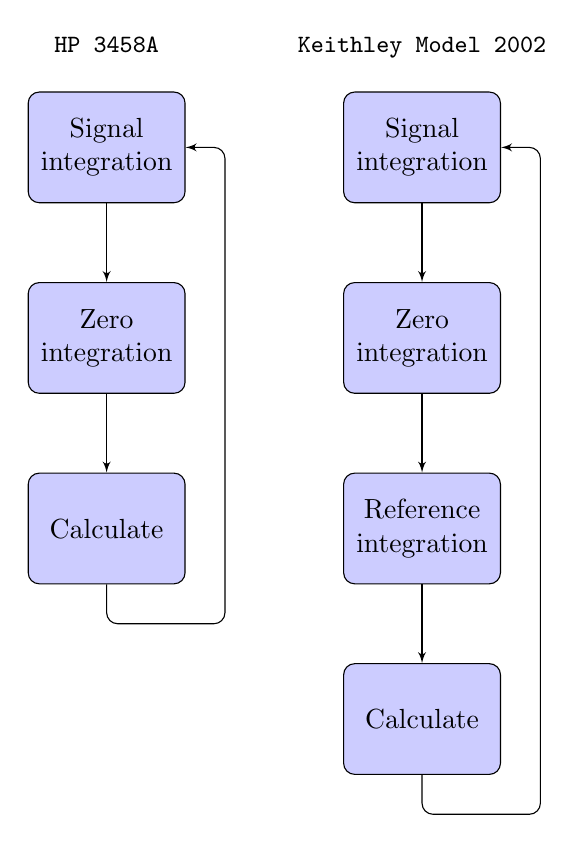
\begin{tikzpicture}[node distance=1cm and 2cm, auto]
        %HP 3458A
        \node [block]  (signal)  {Signal integration};
        \node [above=0.5cm of signal, anchor=base] {\texttt{\small{HP 3458A}}};
        \node [block, below=of signal]  (zero) {Zero integration};
        \node [block, below=of zero] (calculate) {Calculate};
        \path [line] (signal)  -- (zero);
        \path [line] (zero) -- (calculate);
        \path [line,rounded corners] (calculate) |- ($(calculate.south east) + (0.5,-0.5)$) |- (signal);

        % K2002
        \node [block, right=of signal]  (signal)  {Signal integration};
        \node [above=0.5cm of signal, anchor=base] {\texttt{\small{Keithley Model 2002}}};
        \node [block, below=of signal]  (zero) {Zero integration};
        \node [block, below=of zero]  (reference) {Reference integration};
        \node [block, below=of reference] (calculate) {Calculate};
        \path [line] (signal)  -- (zero);
        \path [line] (zero) -- (reference);
        \path [line] (reference) -- (calculate);
        \path [line,rounded corners] (calculate) |- ($(calculate.south east) + (0.5,-0.5)$) |- (signal);
    \end{tikzpicture}
\end{document}
